\documentclass{article}
\usepackage{graphicx}
\usepackage{amsmath}
\usepackage{float}

\title{EDC Assignment 4}
\author{S A Aravind Eswar}

\begin{document}

\maketitle

The circuit is the following,

\begin{figure}[H]
    \centering
    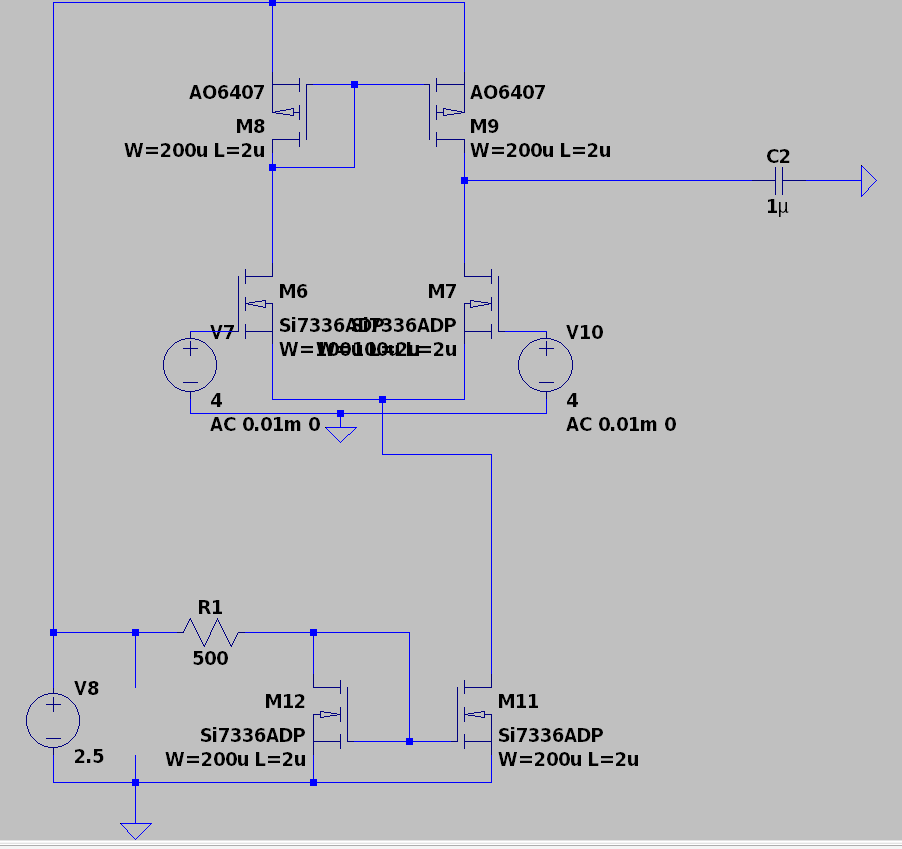
\includegraphics[width=0.75\linewidth]{Differential.jpg}
\end{figure}

\subsection{Small Signal Differential Gain}

In simulation,

At frequency of $200mHz$ with an AC amplitude of $75\mu V$

$common\ gain = 431\mu$

$differential\ gain = 1.75k$

$CMRR = 72.3dB$

$r_o = 796k\Omega$

$g_m = 2.43m\Omega^{-1}$

Input offset voltage = 2.32V

Frequency response,

\begin{figure}[H]
    \centering
    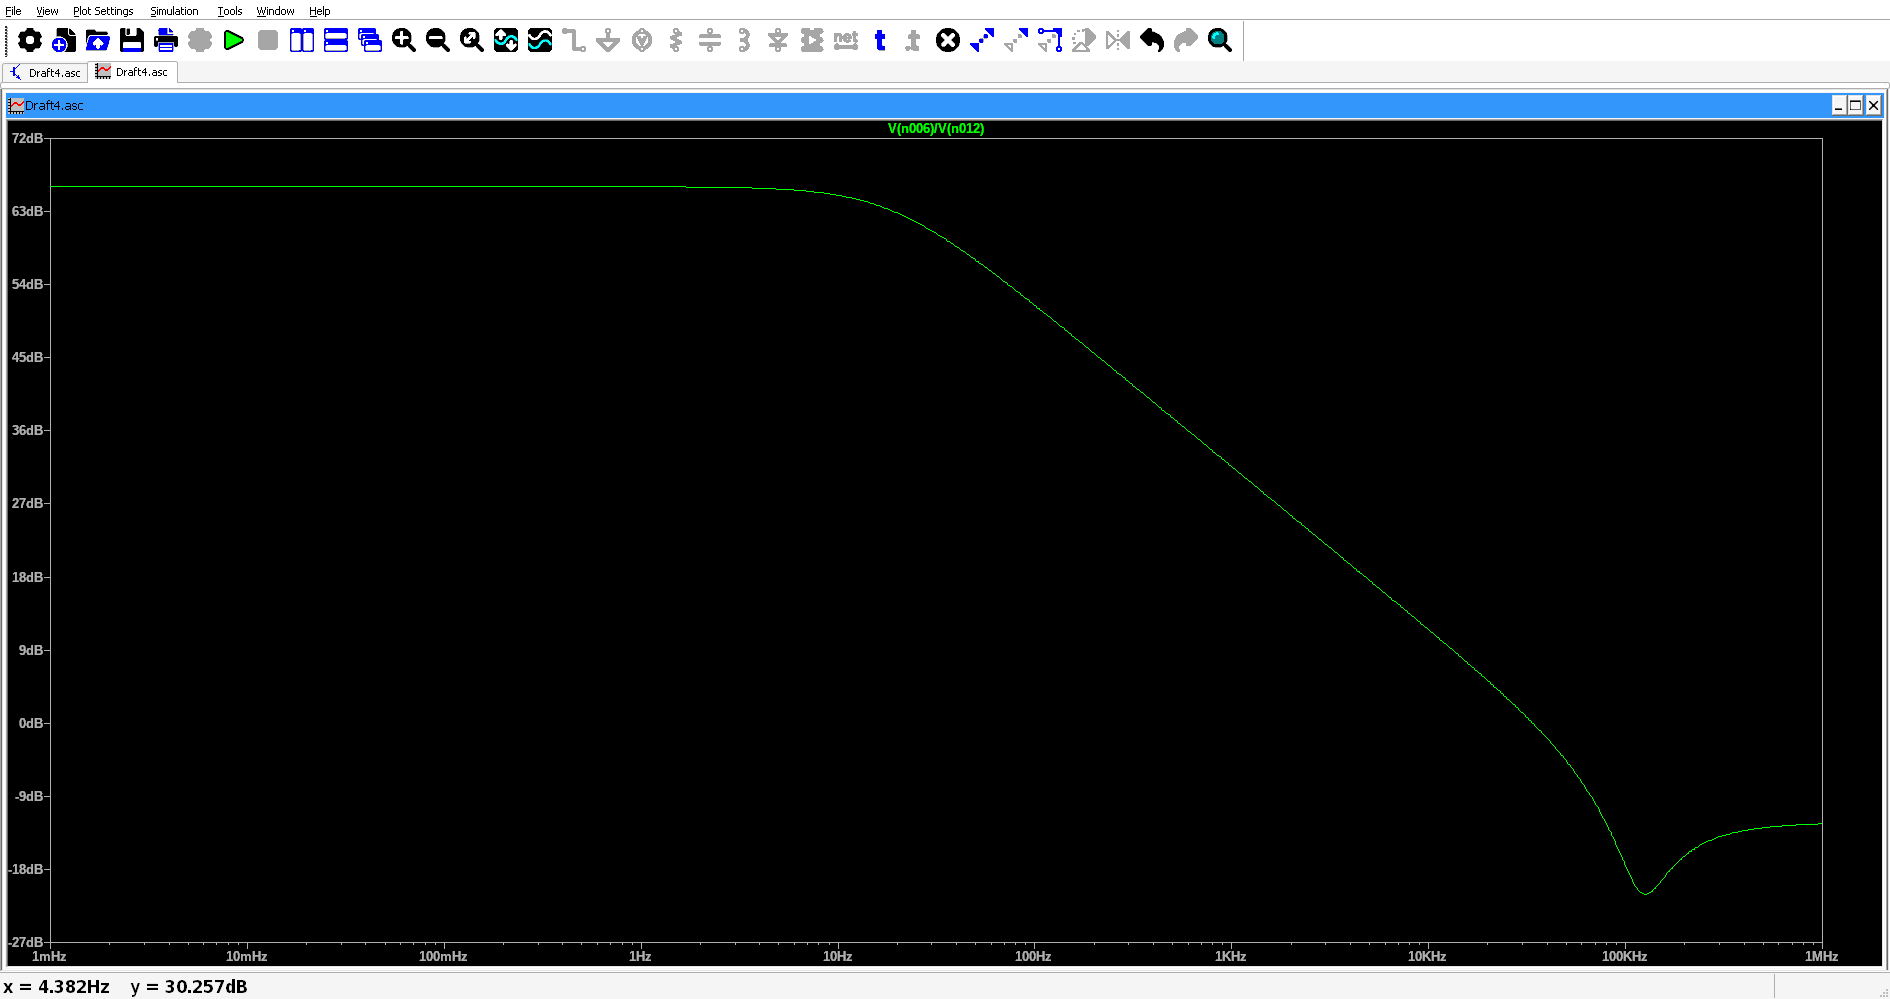
\includegraphics[width=0.75\linewidth]{Frequency.jpg}
\end{figure}

$V_{out}$ for $V_{comm} = 4$ and $ V_{diff} = 75\mu V$ sinusoid of frequency $5Hz$,

\begin{figure}[H]
    \centering
    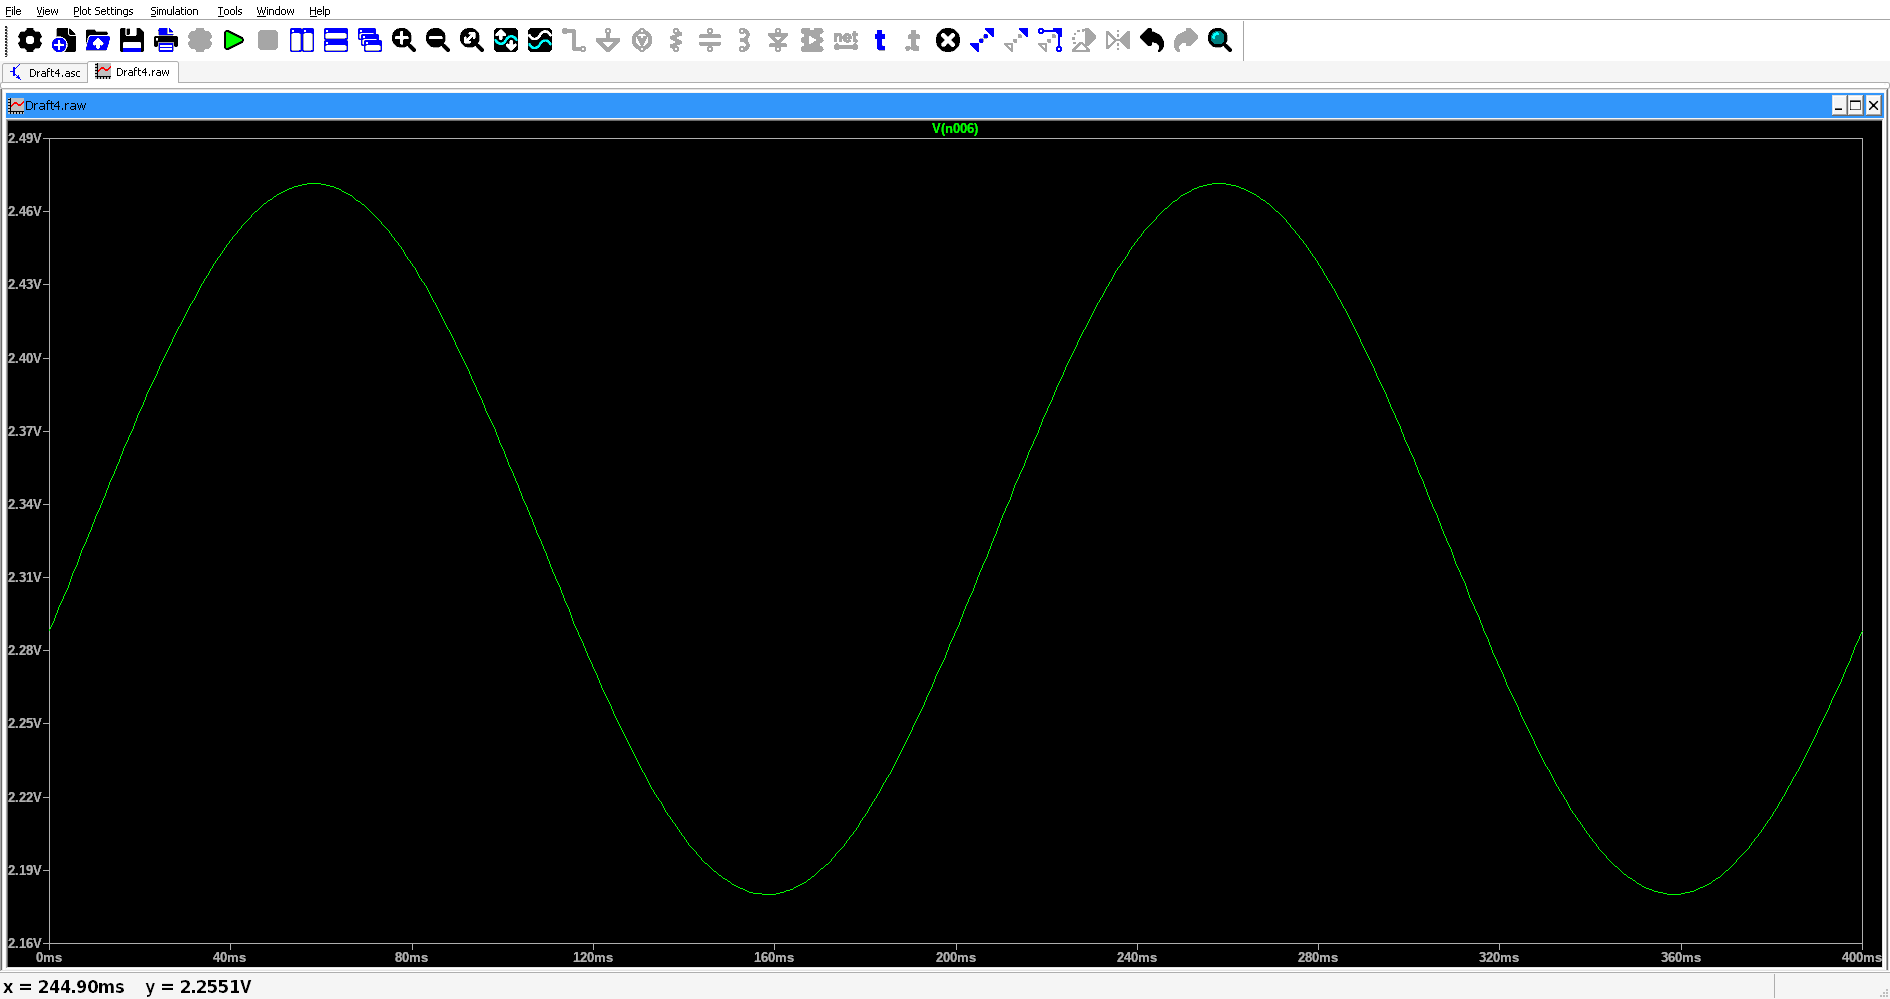
\includegraphics[width=0.75\linewidth]{SmallSignal.jpg}
\end{figure}

Common Mode DC Sweep,

\begin{figure}[H]
    \centering
    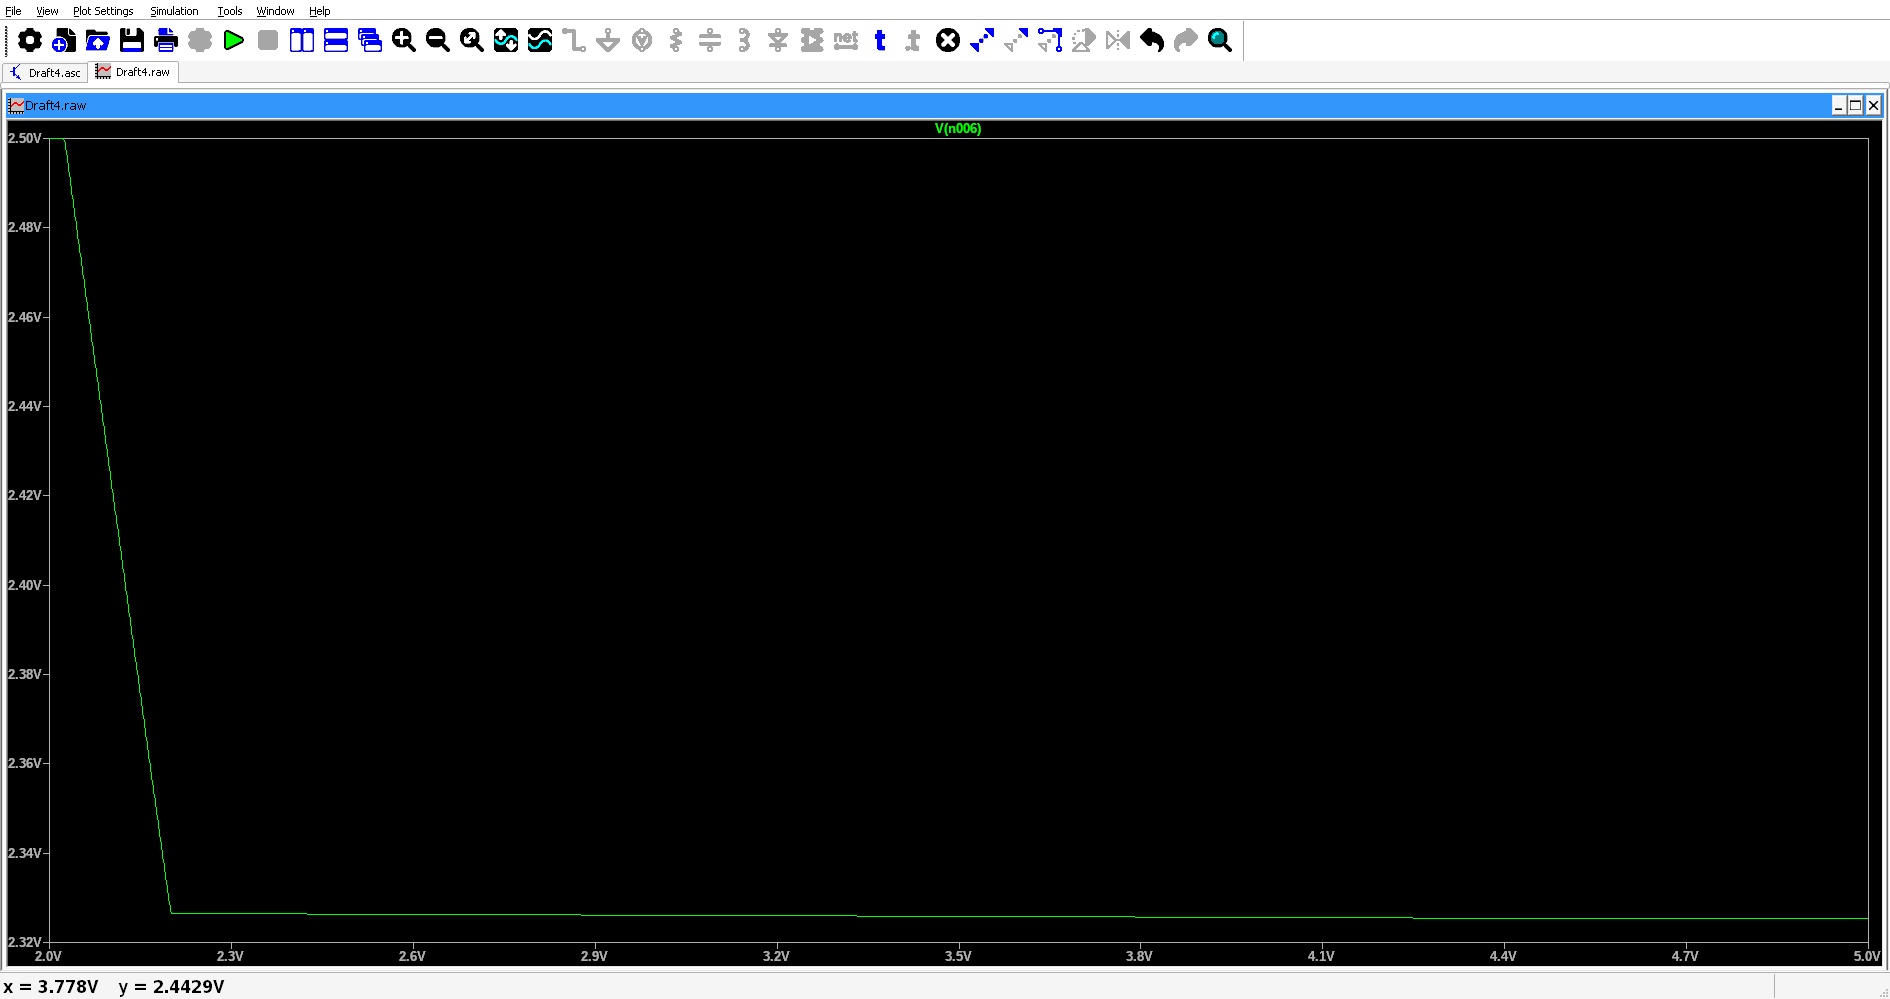
\includegraphics[width=0.75\linewidth]{CommonDC.jpg}
\end{figure}

Differential Mode DC Sweep,

\begin{figure}[H]
    \centering
    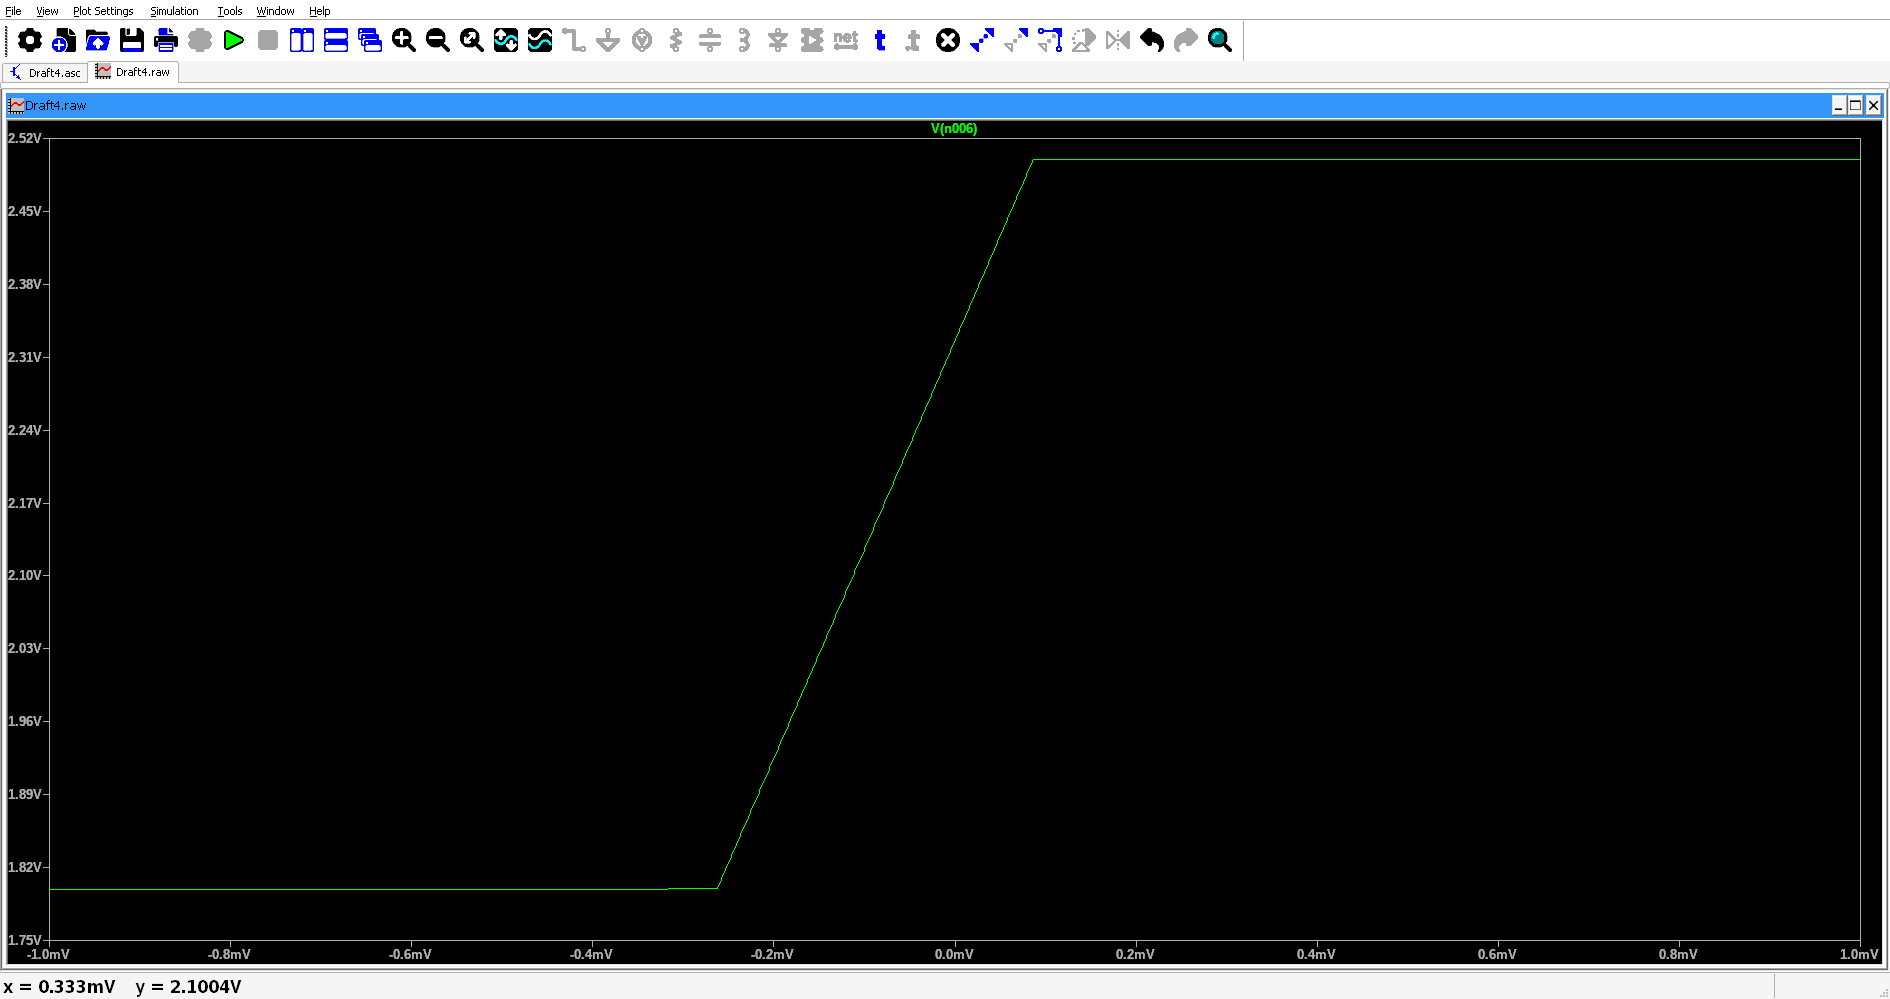
\includegraphics[width=0.75\linewidth]{DifferenceDC.jpg}
\end{figure}

Theoretical Calculations for gain,

differential gain = $g_m(r_{o_n}||r_{o_p})$


$r_{o_n} = \frac{1}{\lambda I_D} = 434.8k\Omega$
$r_{o_p} = \infty$ as $\lambda = 0$

Thus,

$gain = 1k$

\end{document}
